% Options for packages loaded elsewhere
% Options for packages loaded elsewhere
\PassOptionsToPackage{unicode}{hyperref}
\PassOptionsToPackage{hyphens}{url}
%
\documentclass[
  10pt,
  ignorenonframetext,
  aspectratio=169,
  spanish,
]{beamer}
\newif\ifbibliography
\usepackage{pgfpages}
\setbeamertemplate{caption}[numbered]
\setbeamertemplate{caption label separator}{: }
\setbeamercolor{caption name}{fg=normal text.fg}
\beamertemplatenavigationsymbolsempty
% remove section numbering
\setbeamertemplate{part page}{
  \centering
  \begin{beamercolorbox}[sep=16pt,center]{part title}
    \usebeamerfont{part title}\insertpart\par
  \end{beamercolorbox}
}
\setbeamertemplate{section page}{
  \centering
  \begin{beamercolorbox}[sep=12pt,center]{section title}
    \usebeamerfont{section title}\insertsection\par
  \end{beamercolorbox}
}
\setbeamertemplate{subsection page}{
  \centering
  \begin{beamercolorbox}[sep=8pt,center]{subsection title}
    \usebeamerfont{subsection title}\insertsubsection\par
  \end{beamercolorbox}
}
% Prevent slide breaks in the middle of a paragraph
\widowpenalties 1 10000
\raggedbottom
\AtBeginPart{
  \frame{\partpage}
}
\AtBeginSection{
  \ifbibliography
  \else
    \frame{\sectionpage}
  \fi
}
\AtBeginSubsection{
  \frame{\subsectionpage}
}
\usepackage{iftex}
\ifPDFTeX
  \usepackage[T1]{fontenc}
  \usepackage[utf8]{inputenc}
  \usepackage{textcomp} % provide euro and other symbols
\else % if luatex or xetex
  \usepackage{unicode-math} % this also loads fontspec
  \defaultfontfeatures{Scale=MatchLowercase}
  \defaultfontfeatures[\rmfamily]{Ligatures=TeX,Scale=1}
\fi
\usepackage{lmodern}

\usetheme[]{default}
\usecolortheme[]{dove}
\ifPDFTeX\else
  % xetex/luatex font selection
\fi
% Use upquote if available, for straight quotes in verbatim environments
\IfFileExists{upquote.sty}{\usepackage{upquote}}{}
\IfFileExists{microtype.sty}{% use microtype if available
  \usepackage[]{microtype}
  \UseMicrotypeSet[protrusion]{basicmath} % disable protrusion for tt fonts
}{}
\makeatletter
\@ifundefined{KOMAClassName}{% if non-KOMA class
  \IfFileExists{parskip.sty}{%
    \usepackage{parskip}
  }{% else
    \setlength{\parindent}{0pt}
    \setlength{\parskip}{6pt plus 2pt minus 1pt}}
}{% if KOMA class
  \KOMAoptions{parskip=half}}
\makeatother


\usepackage{longtable,booktabs,array}
\newcounter{none} % for unnumbered tables
\usepackage{calc} % for calculating minipage widths
\usepackage{caption}
% Make caption package work with longtable
\makeatletter
\def\fnum@table{\tablename~\thetable}
\makeatother
\usepackage{graphicx}
\makeatletter
\newsavebox\pandoc@box
\newcommand*\pandocbounded[1]{% scales image to fit in text height/width
  \sbox\pandoc@box{#1}%
  \Gscale@div\@tempa{\textheight}{\dimexpr\ht\pandoc@box+\dp\pandoc@box\relax}%
  \Gscale@div\@tempb{\linewidth}{\wd\pandoc@box}%
  \ifdim\@tempb\p@<\@tempa\p@\let\@tempa\@tempb\fi% select the smaller of both
  \ifdim\@tempa\p@<\p@\scalebox{\@tempa}{\usebox\pandoc@box}%
  \else\usebox{\pandoc@box}%
  \fi%
}
% Set default figure placement to htbp
\def\fps@figure{htbp}
\makeatother



\ifLuaTeX
\usepackage[bidi=basic,shorthands=off]{babel}
\else
\usepackage[bidi=default,shorthands=off]{babel}
\fi
\ifLuaTeX
  \usepackage{selnolig} % disable illegal ligatures
\fi


\setlength{\emergencystretch}{3em} % prevent overfull lines

\providecommand{\tightlist}{%
  \setlength{\itemsep}{0pt}\setlength{\parskip}{0pt}}



 


\usepackage{booktabs}
\usepackage{caption}
\captionsetup{font=scriptsize}
% --- Paleta ---
\definecolor{acc}{RGB}{123,60,140}
\definecolor{acc2}{RGB}{40,90,130}
\setbeamercolor{frametitle}{fg=white,bg=acc}
\setbeamercolor{title}{fg=acc}
\setbeamercolor{structure}{fg=acc}
\setbeamercolor{alerted text}{fg=acc2}
\setbeamercolor{block title}{fg=white,bg=acc2}
\setbeamercolor{block body}{bg=acc2!8}
\setbeamercolor{block title alerted}{fg=white,bg=acc}
\setbeamercolor{block body alerted}{bg=acc!8}
% --- Tipografía y layout ---
\setbeamerfont{frametitle}{size=\large,series=\bfseries}
\setbeamertemplate{navigation symbols}{}
\setbeamertemplate{footline}[frame number]
\setbeamertemplate{itemize item}{\color{acc}$\bullet$}
\setbeamertemplate{itemize subitem}{\color{acc}--}
\setbeamertemplate{section page}{
  \begin{centering}\vfill
  {\usebeamerfont{section title}\usebeamercolor[fg]{acc}%
   \Large\bfseries\insertsection\par}
  \vfill\end{centering}}
\AtBeginSection[]{\frame{\sectionpage}}
\makeatletter
\@ifpackageloaded{caption}{}{\usepackage{caption}}
\AtBeginDocument{%
\ifdefined\contentsname
  \renewcommand*\contentsname{Tabla de contenidos}
\else
  \newcommand\contentsname{Tabla de contenidos}
\fi
\ifdefined\listfigurename
  \renewcommand*\listfigurename{Listado de Figuras}
\else
  \newcommand\listfigurename{Listado de Figuras}
\fi
\ifdefined\listtablename
  \renewcommand*\listtablename{Listado de Tablas}
\else
  \newcommand\listtablename{Listado de Tablas}
\fi
\ifdefined\figurename
  \renewcommand*\figurename{Figura}
\else
  \newcommand\figurename{Figura}
\fi
\ifdefined\tablename
  \renewcommand*\tablename{Tabla}
\else
  \newcommand\tablename{Tabla}
\fi
}
\@ifpackageloaded{float}{}{\usepackage{float}}
\floatstyle{ruled}
\@ifundefined{c@chapter}{\newfloat{codelisting}{h}{lop}}{\newfloat{codelisting}{h}{lop}[chapter]}
\floatname{codelisting}{Listado}
\newcommand*\listoflistings{\listof{codelisting}{Listado de Listados}}
\makeatother
\makeatletter
\makeatother
\makeatletter
\@ifpackageloaded{caption}{}{\usepackage{caption}}
\@ifpackageloaded{subcaption}{}{\usepackage{subcaption}}
\makeatother

\usepackage{bookmark}
\IfFileExists{xurl.sty}{\usepackage{xurl}}{} % add URL line breaks if available
\urlstyle{same}
% fallback for those not using the hyperref driver hyperxmp:
\makeatletter
\@ifundefined{xmpquote}{\newcommand{\xmpquote}[1]{#1}}{}
\makeatother
\hypersetup{
  pdftitle={¿Son insulares las provincias italianas?},
  pdfauthor={Paula (pau) · Fernando (fer) · Mateo (teo)},
  pdflang={es},
  hidelinks,
  pdfcreator={LaTeX via pandoc}}


\title{\texorpdfstring{¿Son insulares las provincias
italianas?}{¿Son insulares las provincias italianas?}}
\subtitle{\texorpdfstring{Una extensión espacial al multiplicador fiscal
de Acconcia, Corsetti y Simonelli
(2014)}{Una extensión espacial al multiplicador fiscal de Acconcia, Corsetti y Simonelli (2014)}}
\author{Paula (pau) · Fernando (fer) · Mateo (teo)}
\date{Invalid Date}
\institute{Econometría Avanzada II --- Universidad EAFIT}

\begin{document}
\frame{\titlepage}


\section{El problema}\label{el-problema}

\begin{frame}{Medir el multiplicador fiscal es difícil}
\protect\phantomsection\label{medir-el-multiplicador-fiscal-es-difuxedcil}
\textbf{La pregunta:} ¿cuánto cambia el producto local cuando cambia el
gasto público?

\vspace{0.4cm}

\textbf{El obstáculo: el gasto es endógeno.}

\vspace{0.2cm}

\begin{itemize}
\tightlist
\item
  La inversión en infraestructura se \textbf{planea años antes} de
  ejecutarse \newline \(\rightarrow\) efectos de anticipación sesgan el
  multiplicador hacia abajo
\item
  El gobierno \textbf{asigna fondos en respuesta} a la evolución local
  \newline \(\rightarrow\) si compensa provincias rezagadas, MCO
  subestima
\end{itemize}

\vspace{0.4cm}

Ambos sesgos apuntan a cero. Se necesita variación en el gasto que sea
\textbf{ajena al ciclo económico local}.
\end{frame}

\begin{frame}{El experimento natural: Ley 164/1991}
\protect\phantomsection\label{el-experimento-natural-ley-1641991}
\begin{columns}[T]
\begin{column}{0.57\linewidth}
\textbf{Tres piezas institucionales}

\vspace{0.2cm}

\small

\begin{enumerate}
\tightlist
\item
  El gobierno central financia, pero los municipios \textbf{eligen
  proyectos y contratistas}. Sin poder tributario local, el gasto no se
  acompaña de cambios impositivos.
\item
  La obra pública se vuelve negocio central para las mafias.
\item
  \textbf{D.L. 164/1991}: ante evidencia de infiltración se disuelve el
  concejo completo y tres comisarios externos gobiernan 18 meses.
\end{enumerate}

\normalsize

\vspace{0.25cm}

Los comisarios \textbf{cortan el gasto en obra pública}: la contracción
promedio es cercana a 20 p.p. de la inversión.
\end{column}

\begin{column}{0.43\linewidth}
\pandocbounded{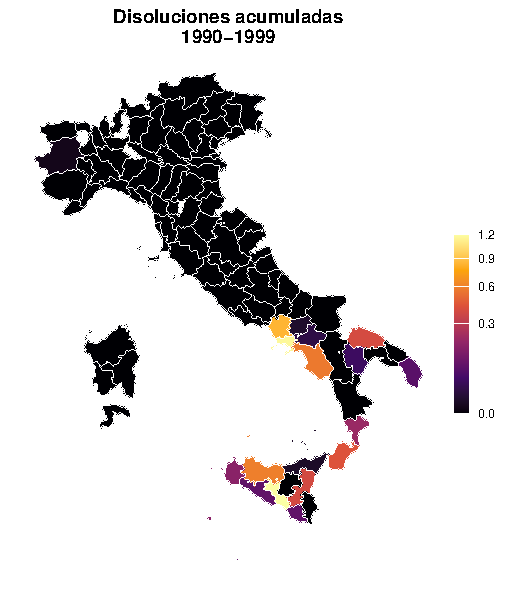
\includegraphics[keepaspectratio]{presentacion_files/figure-beamer/unnamed-chunk-1-1.pdf}}
\end{column}
\end{columns}
\end{frame}

\begin{frame}{Datos y especificación}
\protect\phantomsection\label{datos-y-especificaciuxf3n}
\[Y_{i,t} = \beta\, G_{i,t} + \alpha_i + \lambda_t + \gamma X_{i,t} + v_{i,t}\]

\vspace{0.2cm}

\textbf{Panel:} 95 provincias \(\times\) 1990--1999 = 950 observaciones

\vspace{0.2cm}

\small

{\def\LTcaptype{none} % do not increment counter
\begin{longtable}[]{@{}
  >{\raggedright\arraybackslash}p{(\linewidth - 2\tabcolsep) * \real{0.5000}}
  >{\raggedright\arraybackslash}p{(\linewidth - 2\tabcolsep) * \real{0.5000}}@{}}
\toprule\noalign{}
\endhead
\(Y_{i,t}\) & Crecimiento del valor agregado real per cápita \\
\(G_{i,t}\) & \(\Delta\) inversión pública per cápita
\(/\ y_{i,t-1}\) \\
\(CDS1_{i,t}\) & Disoluciones decretadas en el 1er semestre (pond.
población) \\
\(CDS2_{i,t-1}\) & Disoluciones con \$\textless\$180 días hasta fin de
año, rezagadas \\
\bottomrule\noalign{}
\end{longtable}
}

\normalsize

\vspace{0.3cm}

\textbf{Controles:} cinco variables de criminalidad y corrupción con dos
rezagos, dos proxies laborales, rezagos de disoluciones y de \(G\).

\textbf{Decisiones del original que replicamos:} ponderación por
población y errores agrupados región \(\times\) año (190 clusters).
\end{frame}

\section{Parte I --- La replicación}\label{parte-i-la-replicaciuxf3n}

\begin{frame}{Replicamos la Tabla 4 del paper}
\protect\phantomsection\label{replicamos-la-tabla-4-del-paper}
\begin{table}[!h]
\centering\begingroup\fontsize{8}{10}\selectfont

\begin{tabular}[t]{lrrrr}
\toprule
  & OLS & 2SLS & 2SLS + Y rez. & Paper\\
\midrule
$G(t)$ & 0.20** & 1.47*** & 1.55*** & 1.46 / 1.55\\
$G(t-1)$ & 0.21** & 0.73*** & 0.79*** & 0.73 / 0.79\\
$Y(t-1)$ & --- & --- & -0.20*** & $-0.20$\\
$CDS1(t)$ --- 1\textsuperscript{a} etapa & --- & -2.14*** & -2.14*** & $-2.07$\\
$CDS2(t-1)$ --- 1\textsuperscript{a} etapa & --- & -3.98*** & -3.98*** & $-4.02$\\
F instrumentos & --- & 12.80 & 12.82 & 12.58 / 11.83\\
\bottomrule
\end{tabular}
\endgroup{}
\end{table}

\vspace{0.2cm}

\small

\begin{itemize}
\tightlist
\item
  El estimador IV es \textbf{siete veces} el MCO \(\rightarrow\) el
  sesgo de endogeneidad es enorme
\item
  Instrumentos fuertes (F = 12.8), Wu--Hausman rechaza exogeneidad,
  Sargan no rechaza
\item
  Coincidimos con el paper \textbf{hasta en los errores estándar}
\end{itemize}

\normalsize
\end{frame}

\begin{frame}{Los tres multiplicadores}
\protect\phantomsection\label{los-tres-multiplicadores}
\begin{table}[!h]
\centering\begingroup\fontsize{9}{11}\selectfont

\begin{tabular}[t]{lrr}
\toprule
Multiplicador & Nuestro & Paper\\
\midrule
Impacto: $\beta$ & 1.55 & 1.55\\
Dinámico (2 años): $\beta/(1-\phi_1)$ & 1.30 & 1.29\\
Acumulado: $(\beta+\beta_{G,t-1})/(1-\phi_1)$ & 1.96 & 1.95\\
\bottomrule
\end{tabular}
\endgroup{}
\end{table}

\vspace{0.5cm}

\begin{alertblock}{Interpretación}
Un recorte exógeno de inversión pública equivalente al 1\% del valor agregado local reduce el producto provincial en \textbf{1.55\%} el mismo año y hasta \textbf{1.96\%} de forma acumulada.
\end{alertblock}
\end{frame}

\section{Parte II --- La extensión
espacial}\label{parte-ii-la-extensiuxf3n-espacial}

\begin{frame}{La brecha que llenamos}
\protect\phantomsection\label{la-brecha-que-llenamos}
\textbf{Lo que hace el paper (Sección V.A):} añade \(SG_{i,t}\) ---
gasto agregado de las otras provincias de la \textbf{misma región
administrativa} --- como regresor. Concluye que la evidencia de derrames
es ``débil'' y que las provincias son \textbf{insulares}.

\vspace{0.3cm}

\textbf{Cinco limitaciones de ese procedimiento:}

\small

\begin{enumerate}
\tightlist
\item
  Vecindad \textbf{administrativa}, no geográfica (Reggio Calabria y
  Messina: 3 km, regiones distintas)
\item
  Pesos implícitos uniformes dentro de la región
\item
  No modela dependencia en la variable dependiente (\(WY\))
\item
  No modela dependencia en los errores (\(W\varepsilon\))
\item
  No permite descomponer en efectos directo, indirecto y total
\end{enumerate}

\normalsize

\vspace{0.3cm}

\begin{quotation}
\small
``Su estudio requiere una especificación cuidadosa \dots de \textbf{modelos espaciales} que den cuenta de la movilidad transfronteriza de capital y trabajo. Esta es una \textbf{nueva dirección prometedora} para la investigación.''
\hfill --- Acconcia et al. (2014), conclusiones
\end{quotation}
\end{frame}

\begin{frame}{Tests LM: ¿hay dependencia espacial?}
\protect\phantomsection\label{tests-lm-hay-dependencia-espacial}
\begin{table}[!h]
\centering\begingroup\fontsize{9}{11}\selectfont

\begin{tabular}[t]{lr}
\toprule
Test & Estadístico\\
\midrule
LM-lag & 487.86 (p=0.000)\\
LM-error & 438.67 (p=0.000)\\
\textbf{LM-lag robusto} & 64.50 (p=0.000)\\
\textbf{LM-error robusto} & 15.31 (p=0.000)\\
\bottomrule
\end{tabular}
\endgroup{}
\end{table}

\vspace{0.35cm}

Los cuatro tests rechazan: hay dependencia espacial \textbf{tanto en la
variable dependiente como en los errores}, y ambas sobreviven a las
versiones robustas.

\vspace{0.2cm}

\begin{block}{Qué implica}
El protocolo de Elhorst (2010) señala en este caso una especificación \textbf{SARAR} --- rezago espacial de la dependiente \emph{y} autocorrelación en los errores.

\vspace{0.15cm}

Eso motiva directamente nuestro estimador de referencia: el \textbf{SARAR-GMM con instrumentos}.
\end{block}
\end{frame}

\begin{frame}[fragile]{Modelos espaciales: ML frente a GMM}
\protect\phantomsection\label{modelos-espaciales-ml-frente-a-gmm}
\begin{table}[!h]
\centering\begingroup\fontsize{8}{10}\selectfont

\begin{tabular}[t]{lrrc}
\toprule
Modelo & $G(t)$ & $\lambda$ / $\rho$ & Corrige endog.\\
\midrule
SAR (ML) & 0.149*** & 0.407*** & No\\
SEM (ML) & 0.126** & 0.423*** & No\\
SDM (ML) & 0.141** & 0.341*** & No\\
\textbf{SAR-GMM (IV)} & 0.512** & 0.576*** & \textbf{Sí}\\
\textbf{SARAR-GMM (IV)} & 0.299 & 0.935*** & \textbf{Sí}\\
\bottomrule
\end{tabular}
\endgroup{}
\end{table}

\vspace{0.25cm}

\small

\alert{Advertencia clave:} \texttt{splm::spml} \textbf{no admite
instrumentos}. Los modelos ML tratan \(G\) como exógena y reproducen el
sesgo de atenuación: sus coeficientes (0.13--0.15) están más cerca del
MCO (0.20) que del 2SLS (1.55).

\vspace{0.2cm}

El \textbf{GMM de Kelejian--Prucha} (\texttt{spgm}) sí acepta
instrumentos. Al reintroducirlos el coeficiente se recupera, \(\lambda\)
sigue significativo, pero \textbf{no emerge un derrame nítidamente
estimado}.

\normalsize
\end{frame}

\begin{frame}{Heterogeneidad: dónde está la identificación}
\protect\phantomsection\label{heterogeneidad-duxf3nde-estuxe1-la-identificaciuxf3n}
\begin{table}[!h]
\centering\begingroup\fontsize{9}{11}\selectfont

\begin{tabular}[t]{lrrrr}
\toprule
Región & Provincias & Obs & Obs. con instr. $\neq 0$ & $G(t)$\\
\midrule
Norte & 41 & 410 & 1 & -27.38\\
Centro & 20 & 200 & 0 & no identificado\\
Mezzogiorno & 34 & 340 & 40 & 1.20*\\
\bottomrule
\end{tabular}
\endgroup{}
\end{table}

\vspace{0.35cm}

\begin{alertblock}{}
En todo el \textbf{Norte} de Italia, durante los diez años, hay \textbf{una sola} observación provincia--año con instrumento distinto de cero. En el \textbf{Centro}, ninguna.

\vspace{0.15cm}

Toda la variación instrumental está en el Mezzogiorno --- y el multiplicador allí reproduce el de la muestra completa. Es la contrapartida exacta de un diseño de LATE, y \textbf{valida el diseño}.
\end{alertblock}
\end{frame}

\begin{frame}{Síntesis: lo que discrimina los resultados}
\protect\phantomsection\label{suxedntesis-lo-que-discrimina-los-resultados}
\begin{table}[!h]
\centering\begingroup\fontsize{8}{10}\selectfont

\begin{tabular}[t]{lrcc}
\toprule
Modelo & $G(t)$ & Endog. & Espacio\\
\midrule
OLS ponderado & 0.20 & No & No\\
\textbf{2SLS} & \textbf{1.47} & Sí & No\\
\textbf{2SLS + Y rez.} & \textbf{1.55} & Sí & No\\
SAR (ML) & 0.149*** & No & Sí\\
SEM (ML) & 0.126** & No & Sí\\
SDM (ML) & 0.141** & No & Sí\\
SAR-GMM & 0.512** & Sí & Sí\\
SARAR-GMM & 0.299 & Sí & Sí\\
2SLS (Mezzogiorno) & 1.20* & Sí & No\\
\bottomrule
\end{tabular}
\endgroup{}
\end{table}

\vspace{0.25cm}

\small

Las especificaciones que \textbf{no} instrumentan entregan 0.13--0.20,
modelen o no el espacio. Las que \textbf{sí} instrumentan: 1.47--1.55
sin estructura espacial, 0.30--0.51 con ella.

\vspace{0.15cm}

\(\Rightarrow\) Lo que discrimina los resultados es \textbf{el
tratamiento de la endogeneidad}, no el del espacio. Y el parámetro
espacial es significativo en todas las especificaciones que lo estiman.

\normalsize
\end{frame}

\section{Conclusiones}\label{conclusiones}

\begin{frame}{La insularidad se sostiene}
\protect\phantomsection\label{la-insularidad-se-sostiene}
\textbf{La evidencia converge desde tres direcciones:}

\vspace{0.2cm}

\begin{enumerate}
\tightlist
\item
  El \textbf{diagnóstico LM} señala una especificación SARAR --- que es
  exactamente la que estimamos por GMM con instrumentos
\item
  El \textbf{SARAR-GMM} confirma dependencia espacial (\(\lambda\)
  significativo) pero \textbf{no} produce un derrame del gasto
  nítidamente estimado
\item
  La \textbf{robustez a cuatro matrices \(W\)} (k-NN 4 y 6, reina,
  distancia inversa) descarta que sea artefacto de la vecindad elegida
\end{enumerate}

\vspace{0.3cm}

\small

Conviene distinguir dos cosas: que el crecimiento de provincias vecinas
esté \textbf{correlacionado} no implica que el \textbf{gasto} de una
mueva el producto de las otras. Lo primero lo confirmamos; lo segundo no
aparece. \normalsize

\vspace{0.4cm}

Confirmamos la conclusión del paper \textbf{sobre una base metodológica
más exigente}: ellos la establecieron con vecindad administrativa y sin
descomposición de efectos; nosotros con geografía explícita, tests
formales, la familia SAR--SEM--SDM e impactos de LeSage--Pace.
\end{frame}

\begin{frame}{Lección metodológica y política}
\protect\phantomsection\label{lecciuxf3n-metodoluxf3gica-y-poluxedtica}
\begin{block}{Metodología}
Aplicar econometría espacial sobre un diseño cuasi-experimental \textbf{sin preservar la estrategia de identificación} reintroduce el sesgo que el diseño existe para eliminar.

\vspace{0.15cm}

Cuando ambas patologías coexisten, el GMM espacial no es un refinamiento opcional: es un requisito.
\end{block}

\vspace{0.3cm}

\begin{block}{Política}
El costo económico de una disolución administrativa se concentra en la jurisdicción intervenida y no se difunde a sus vecinas.

\vspace{0.15cm}

Esto simplifica el diseño de compensaciones --- pueden focalizarse sin coordinación interprovincial --- pero implica que la provincia afectada \textbf{absorbe íntegramente el ajuste}.
\end{block}
\end{frame}

\begin{frame}{\phantom{Gracias}}
\protect\phantomsection\label{section}
\begin{center}
\vspace{1cm}
{\Huge Gracias}

\vspace{1.2cm}

{\large Las tres cifras}

\vspace{0.5cm}

\begin{tabular}{cl}
\textbf{1.55} & multiplicador de impacto \\[0.3cm]
\textbf{1.96} & multiplicador acumulado \\[0.3cm]
\textbf{1} & observación con instrumento $\neq 0$ \\
 & en todo el Norte de Italia \\
\end{tabular}
\end{center}
\end{frame}




\end{document}
